\documentclass[10pt,a4paper]{article}
\usepackage[utf8]{inputenc}
\usepackage[T1]{fontenc}
\usepackage[spanish]{babel}
\usepackage{geometry}
\geometry{a4paper, margin=0.75in, headheight=14pt}
\usepackage{graphicx}
\usepackage{xcolor}
\usepackage{hyperref}
\usepackage{booktabs}
\usepackage{fancyhdr}
\usepackage{titlesec}
\usepackage{listings}
\usepackage{amsmath}
\usepackage{tcolorbox}
\usepackage{enumitem}
\usepackage{float}
\setlength{\abovecaptionskip}{2pt}
\setlength{\belowcaptionskip}{2pt}

% --- Fuente Arial (Helvética) ---
\usepackage{helvet}
\renewcommand{\familydefault}{\sfdefault}

% --- Colores ---
\definecolor{successgreen}{HTML}{10B981}
\definecolor{warnorange}{HTML}{F59E0B}
\definecolor{critred}{HTML}{EF4444}
\definecolor{lightbg}{HTML}{F8FAFC}
\definecolor{bordergray}{HTML}{E2E8F0}

% --- Hipervínculos en negro ---
\hypersetup{
    colorlinks=true,
    linkcolor=black,
    filecolor=black,
    urlcolor=black,
    pdftitle={Manual de Usuario - SmartSaver},
    pdfpagemode=FullScreen,
}

% --- Estilo de Página ---
\pagestyle{fancy}
\fancyhf{}
\fancyhead[L]{\textbf{SmartSaver} --- Manual de Usuario}
\fancyhead[R]{}
\fancyfoot[C]{\thepage}
\renewcommand{\headrulewidth}{0.5pt}
\renewcommand{\footrulewidth}{0.5pt}

% --- Formato de Secciones ---
\titleformat{\section}
  {\color{black}\normalfont\large\bfseries}
  {\thesection}{0.8em}{}
  [\vspace{-0.3em}]
\titleformat{\subsection}
  {\color{black}\normalfont\normalsize\bfseries}
  {\thesubsection}{0.8em}{}
  [\vspace{-0.3em}]
\titlespacing*{\section}{0pt}{1em}{0.5em}
\titlespacing*{\subsection}{0pt}{0.8em}{0.4em}

% --- Cajas de Información ---
\newtcolorbox{infoBox}{
  colback=lightbg,
  colframe=black,
  fonttitle=\bfseries,
  coltitle=white,
  title=Información Importante,
  arc=3pt,
  boxsep=2pt,
  left=4pt,
  right=4pt,
  top=2pt,
  bottom=2pt
}

\newtcolorbox{alertBox}{
  colback=lightbg,
  colframe=critred,
  fonttitle=\bfseries,
  coltitle=white,
  title=Alerta de Seguridad,
  arc=3pt,
  boxsep=2pt,
  left=4pt,
  right=4pt,
  top=2pt,
  bottom=2pt
}

\setlength{\parskip}{2pt}
\setlength{\itemsep}{2pt}

\begin{document}
\pagenumbering{roman}

% ==========================================
% PORTADA
% ==========================================
\begin{titlepage}
    \centering
    \vspace*{1.5cm}
    {\Huge \bfseries \color{black} SMARTSAVER} \\[0.3cm]
    {\large \bfseries \color{black} Sistema integrado para el consumo de energía en artefactos eléctricos mediante inteligencia artificial} \\[1cm]
    \vspace*{1cm}
    
    {\large \textbf{Manual de Usuario Oficial}} \\[0.3cm]
    {\large Versión 1.0} \\[1.5cm]
    
    \textbf{Desarrollado para:} \\
    Monitoreo y gestion de carga en artefactos eléctricos. \\[0.5cm]
    
    \vfill
    {\large Julio 2026}
\end{titlepage}

\setcounter{page}{2}
\tableofcontents
\newpage
\pagenumbering{arabic}

% ==========================================
% SECCIÓN 1: INTRODUCCIÓN
% ==========================================
\section{Introducción}
\textbf{SmartSaver} es una aplicación móvil para monitorear y controlar sistemas de control de carga inteligente. Desde la app puede encender y apagar dispositivos, ver el consumo eléctrico en tiempo real, establecer límites de seguridad, programar horarios de operación y consultar el historial de eventos.

% ==========================================
% SECCIÓN 2: EL SISTEMA
% ==========================================
\section{El Sistema}

\textbf{SmartSaver} es la aplicación móvil del sistema. El sistema completo se compone de dos nodos que trabajan junto a sus fuentes de respaldo de energía (como UPS o baterías de respaldo):

\begin{itemize}
    \item \textbf{Nodo Central (Puerta de Enlace):} Conecta los dispositivos a su red WiFi y sincroniza los datos con la app.
    \item \textbf{Nodo Periférico (Toma Inteligente):} El enchufe físico donde conecta sus artefactos. Mide el consumo eléctrico en tiempo real y puede cortar la corriente automáticamente si detecta una carga peligrosa.
\end{itemize}

\subsection{Configuración del nodo central}
Al encender el nodo central por primera vez, creará su propia red WiFi llamada \textbf{Setup\_Gateway}. Para conectarlo a su red doméstica:

\begin{enumerate}
    \item En su teléfono o computadora, conéctese a la red \textbf{Setup\_Gateway}. La contraseña es \textbf{admin123}.
    \item Abra un navegador web y escriba la dirección \textbf{192.168.4.1}.
    \item Se mostrará una página de configuración. Ingrese el nombre de su red WiFi (SSID) y su contraseña.
    \item Presione el botón para guardar. El nodo central se reiniciará y se conectará automáticamente a su red.
\end{enumerate}

\subsection{Emparejamiento}
Antes del primer uso, cada toma inteligente debe vincularse con el nodo central:

\begin{enumerate}
    \item Asegúrese de que el nodo central esté conectado a su red WiFi.
    \item Enchufe la toma inteligente. Mantenga presionado el botón de emparejamiento hasta que el LED parpadee rápidamente.
    \item En pocos segundos, el LED se quedará fijo. El enlace está completo.
    \item Conecte su artefacto a la toma. El sistema comenzará a monitorearlo de inmediato.
\end{enumerate}

% ==========================================
% SECCIÓN 3: INICIO DE SESIÓN
% ==========================================
\section{Inicio de Sesión}

\subsection{Primer acceso}
\begin{enumerate}
    \item Abra la aplicación.
    \item Presione \textbf{Iniciar Sesión}.
    \item Ingrese su correo y contraseña en la pantalla de autenticación. Se recomienda usar su cuenta de Google para un inicio de sesión más rápido y seguro.
    \item Tras validar sus credenciales, la aplicación lo dirigirá al Dashboard.
\end{enumerate}

\subsection{Configuración inicial}
La primera vez que ingrese, la app le pedirá un nombre o apodo para personalizar los saludos. Puede aceptar el valor sugerido o escribir uno nuevo.

\subsection{Cerrar sesión}
En la pantalla \textbf{Ajustes}, presione \textbf{Cerrar Sesión}. La aplicación borrará los datos locales de sesión y volverá a la pantalla de inicio.

% ==========================================
% SECCIÓN 4: DASHBOARD
% ==========================================
\section{Dashboard}

\begin{figure}[H]
    \centering
    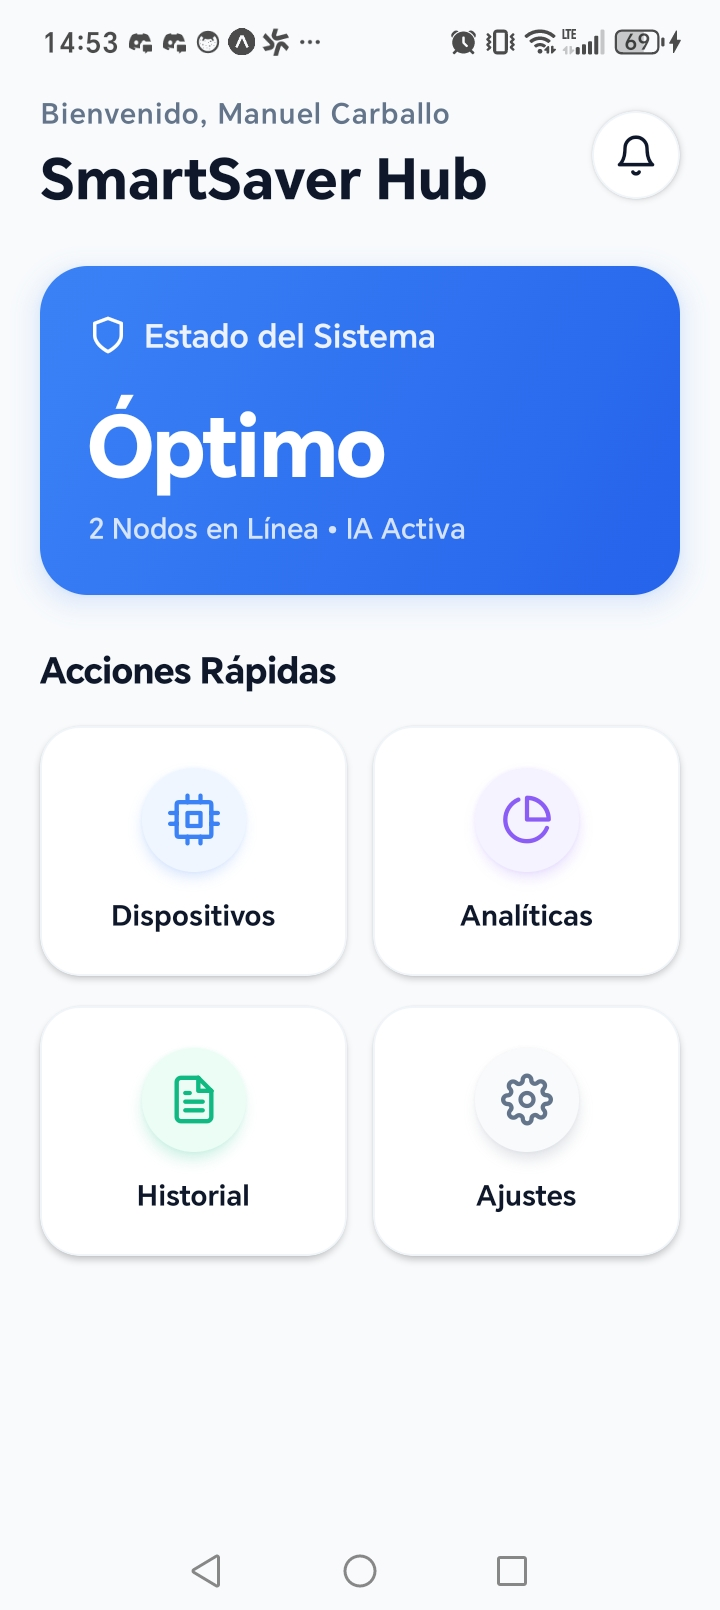
\includegraphics[width=0.28\textwidth]{../aplicacion_ss/HOMESCREEN.jpg}
    \caption{Dashboard del Sistema}
    \label{fig:homescreen}
\end{figure}

El Dashboard es la pantalla principal. Muestra:

\begin{itemize}
    \item \textbf{Saludo personalizado:} "Bienvenido, [Nombre]" y el título \textbf{SmartSaver Hub}.
    \item \textbf{Estado del sistema:} Tarjeta que indica si el sistema está \textit{Óptimo} (hay dispositivos en línea) o \textit{Crítico} (todos fuera de línea). También muestra la cantidad de nodos activos y si la IA está activa.
    \item \textbf{Acciones rápidas:} Cuatro botones de acceso directo:
    \begin{itemize}
        \item \textbf{Dispositivos:} Lista de sistemas de control de carga activos.
        \item \textbf{Analíticas:} Gráficos de consumo y exportación de reportes.
        \item \textbf{Historial:} Bitácora de eventos del sistema.
        \item \textbf{Ajustes:} Configuración global, perfil, modo oscuro y conectividad.
    \end{itemize}
    \item \textbf{Campana de notificaciones:} En la esquina superior derecha. Muestra la cantidad de notificaciones push sin leer. Toque la campana para ver el historial completo de alertas.
\end{itemize}

% ==========================================
% SECCIÓN 5: DISPOSITIVOS ACTIVOS
% ==========================================
\section{Dispositivos Activos}

\begin{figure}[H]
    \centering
    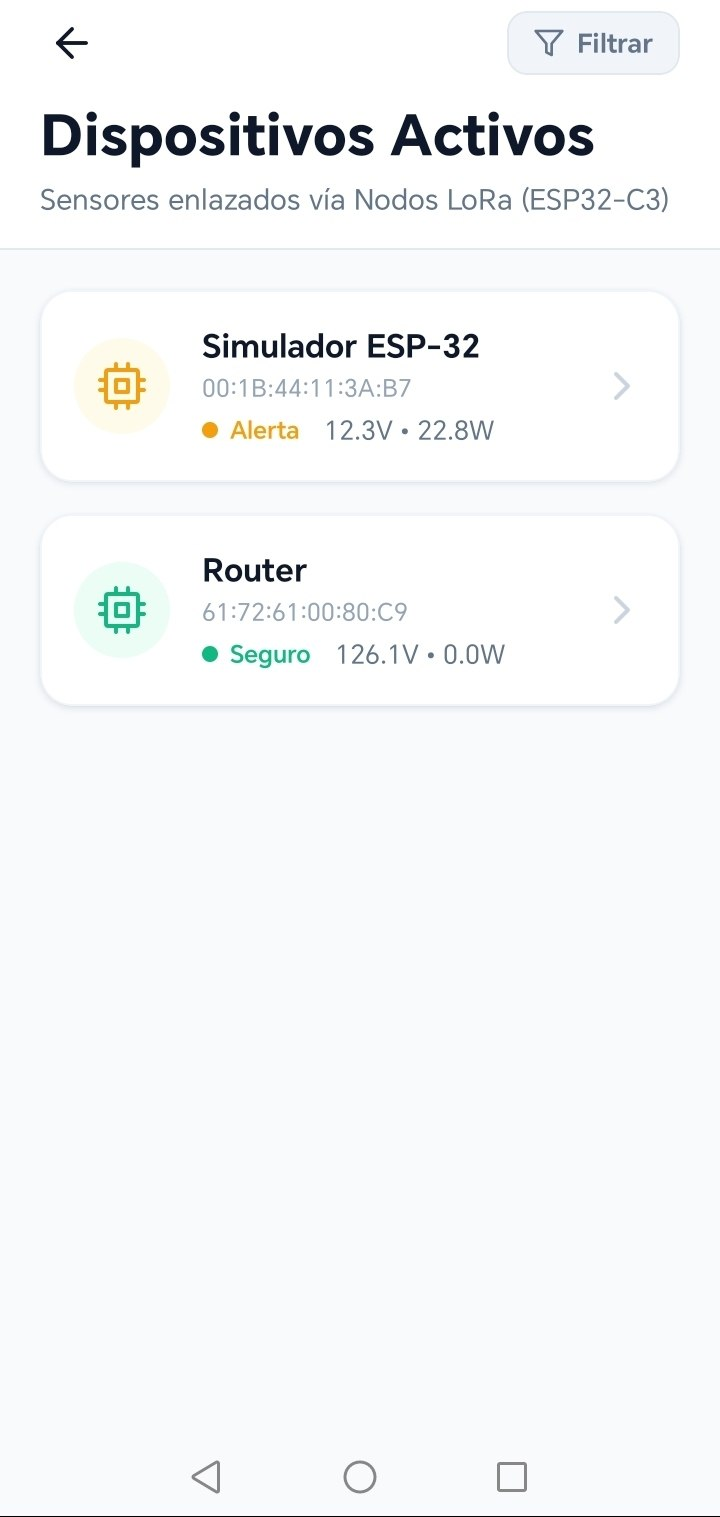
\includegraphics[width=0.28\textwidth]{../aplicacion_ss/ACTIVE_DEVICES.jpg}
    \caption{Lista de Dispositivos Activos}
    \label{fig:active_devices}
\end{figure}

Esta pantalla muestra todos los dispositivos vinculados a su cuenta.

\subsection{Filtros}
En la parte superior hay un botón \textbf{Filtrar} que despliega opciones: \textbf{Todos}, \textbf{P1}, \textbf{P2} y \textbf{P3}. Seleccione una prioridad para mostrar solo los dispositivos de esa categoría.

\subsection{Tarjeta de dispositivo}
Cada dispositivo muestra:
\begin{itemize}
    \item Nombre personalizado (o dirección MAC si no tiene nombre).
    \item Estado de conexión: \textit{Conectado} (verde), \textit{En espera} (gris), \textit{Sincronizando} (amarillo) o \textit{Sin señal} (rojo).
    \item Estado de seguridad de la IA: \textit{Seguro} (verde), \textit{Riesgo} (naranja), \textit{Crítico} (rojo) o \textit{Sin Señal}.
    \item Telemetría en vivo: voltaje y potencia actual (por ejemplo, \textit{12.3V · 22.8W}).
\end{itemize}

\subsection{Editar nombre}
Mantenga presionada la tarjeta de un dispositivo para abrir un cuadro de edición. Escriba el nombre deseado y presione \textbf{Guardar}. Para eliminar el nombre personalizado y volver a la MAC, presione \textbf{Eliminar}.

% ==========================================
% SECCIÓN 6: PANEL DE DETALLE
% ==========================================
\section{Panel de Detalle del Dispositivo}

\begin{figure}[H]
    \centering
    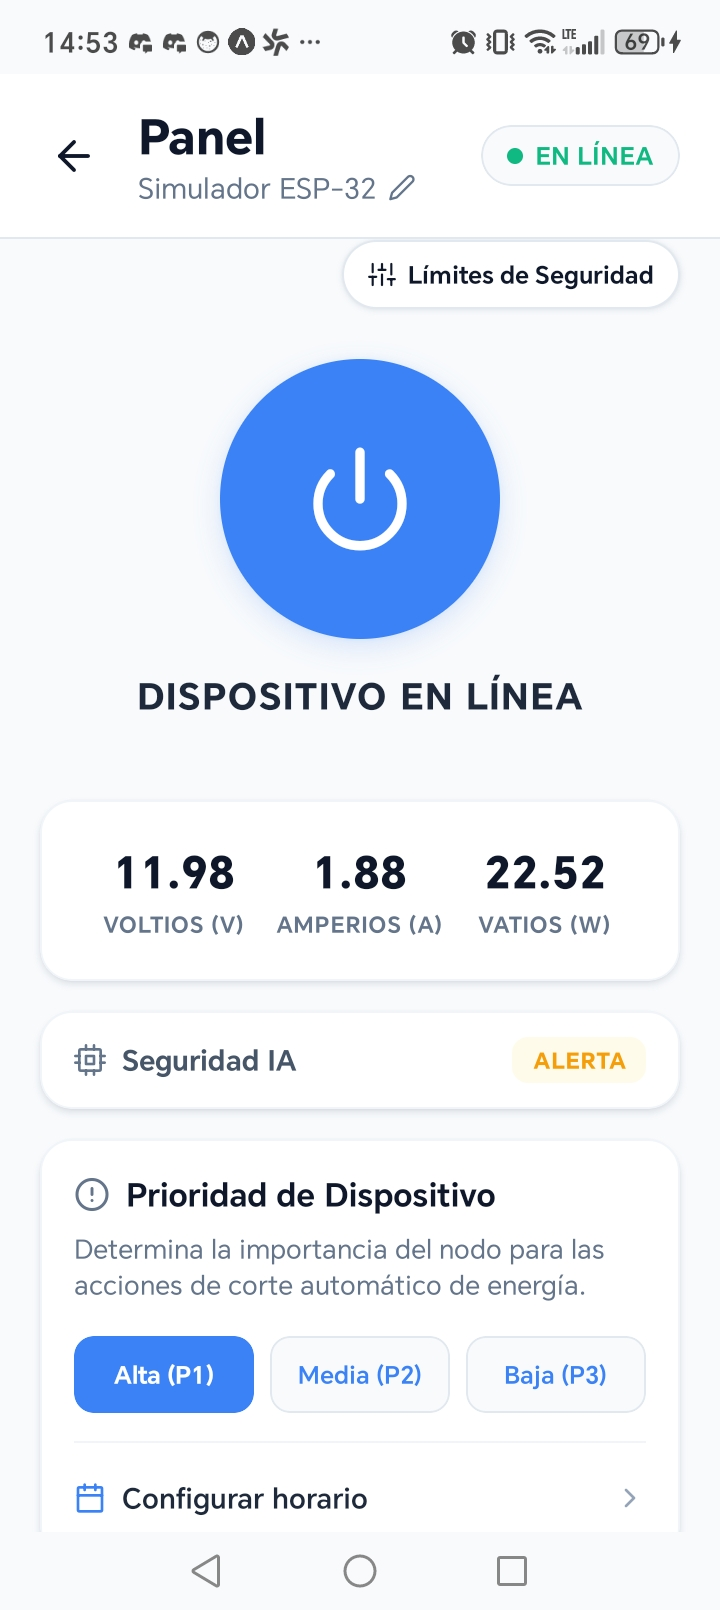
\includegraphics[width=0.28\textwidth]{../aplicacion_ss/DEVICE_SCREEN.jpg}
    \caption{Panel de Detalle}
    \label{fig:device_screen}
\end{figure}

Toque cualquier dispositivo en la lista para abrir su panel de detalle. Aquí controla el dispositivo y revisa su estado.

\subsection{Encabezado}
\begin{itemize}
    \item \textbf{Nombre:} Toque el nombre (o el icono de lápiz) para editarlo.
    \item \textbf{Estado de red:} Píldora verde \textit{En línea} o roja \textit{Off}.
\end{itemize}

\subsection{Botón de encendido/apagado}
En el centro hay un botón circular grande con el símbolo de encendido:
\begin{itemize}
    \item \textbf{Azul brillante:} El dispositivo está encendido.
    \item \textbf{Gris:} El dispositivo está apagado.
    \item \textbf{Desactivado:} Si el dispositivo está fuera de línea, el botón se bloquea en gris y aparece un banner rojo.
\end{itemize}

Debajo del botón se muestra el estado textual:
\begin{itemize}
    \item \textbf{DISPOSITIVO EN LÍNEA:} Funcionando normalmente.
    \item \textbf{DISPOSITIVO DESCONECTADO:} Apagado pero en línea.
    \item \textbf{SINCRONIZANDO...:} Esperando confirmación del dispositivo.
    \item \textbf{ENVIANDO COMANDO...:} La orden está en tránsito.
    \item \textbf{DISPOSITIVO INALCANZABLE:} Sin conexión de red.
\end{itemize}

\begin{alertBox}
Si el dispositivo está fuera de línea, el botón se deshabilita y aparece un banner rojo. No envíe comandos hasta restablecer la conexión.
\end{alertBox}

\smallskip
Si la IA está controlando el dispositivo y usted intenta apagarlo manualmente, aparecerá un diálogo de confirmación. Toque \textbf{Sí, controlar manualmente} para continuar con el apagado.

\subsection{Apagado programado por IA}
Si el sistema detecta un riesgo prolongado, puede mostrar una tarjeta de cuenta regresiva con el tiempo restante antes de un apagado automático. Toque \textbf{Mantener} para posponer el apagado 30 minutos.

\subsection{Alerta BMS crítica}
En caso de una condición crítica (por ejemplo, sobrecalentamiento), el sistema fuerza un apagado preventivo. El panel mostrará \textbf{CRÍTICO} en rojo, una descripción del problema y un botón \textbf{Confirmar} para restablecer la alerta una vez resuelta la causa.

\subsection{Seguridad IA}
Una tarjeta indica la clasificación de riesgo del dispositivo:
\begin{itemize}
    \item \textbf{SEGURO:} Consumo normal.
    \item \textbf{RIESGO:} Consumo elevado.
    \item \textbf{CRÍTICO:} Sobrecarga detectada.
    \item \textbf{SIN SEÑAL / EN ESPERA:} Dispositivo sin conexión o apagado.
\end{itemize}

\subsection{Telemetría}
Tarjeta dividida en tres columnas:
\begin{enumerate}
    \item \textbf{Voltios (V):} Tensión actual.
    \item \textbf{Amperios (A):} Corriente consumida.
    \item \textbf{Vatios (W):} Potencia activa total ($P = V \times I$).
\end{enumerate}

\subsection{Prioridad del dispositivo}
Tarjeta para seleccionar la prioridad del dispositivo:
\begin{itemize}
    \item \textbf{Alta (P1):} Dispositivos críticos. Últimos en apagarse en emergencias.
    \item \textbf{Media (P2):} Prioridad estándar.
    \item \textbf{Baja (P3):} Dispositivos secundarios. Se apagan primero en emergencias.
\end{itemize}

\subsection{Horario de operación}
Dentro de la tarjeta de prioridad, toque \textbf{Configurar horario} para ir a la pantalla de programación.

\subsection{Límites de seguridad}
En la parte superior derecha, toque el botón \textbf{Límites de Seguridad} para abrir la configuración de umbrales eléctricos. Se describe en la siguiente sección.

% ==========================================
% SECCIÓN 7: LÍMITES DE SEGURIDAD
% ==========================================
\section{Límites de Seguridad}

\begin{figure}[H]
    \centering
    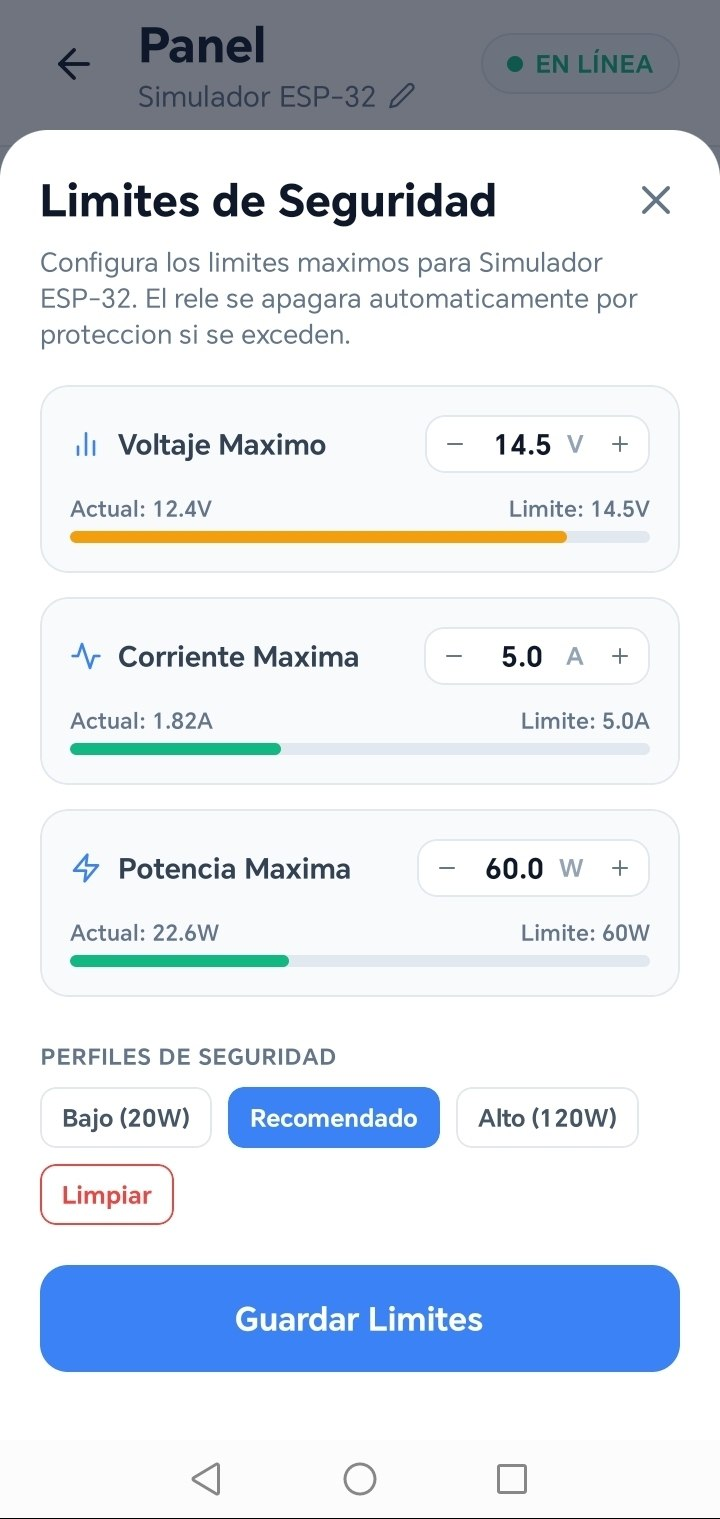
\includegraphics[width=0.28\textwidth]{../aplicacion_ss/ENERGY_LIMITS_SETUP.jpg}
    \caption{Configuración de Límites Eléctricos}
    \label{fig:energy_limits_setup}
\end{figure}

Establezca valores máximos de voltaje, corriente y potencia. Si el dispositivo supera alguno de estos límites, se ejecuta un \textbf{apagado de emergencia automático}.

\subsection{Umbrales disponibles}
\begin{itemize}
    \item \textbf{Voltaje Máximo:} $0.1V$ --- $250V$.
    \item \textbf{Corriente Máxima:} $0.1A$ --- $30A$.
    \item \textbf{Potencia Máxima:} $0.1W$ --- $500W$.
\end{itemize}

\subsection{Formas de ajuste}
\begin{enumerate}
    \item \textbf{Botones +/-:} Toque los botones laterales para ajustar el valor en pasos fijos:
    \begin{itemize}
        \item Voltaje: $\pm 0.5V$.
        \item Corriente: $\pm 0.1A$.
        \item Potencia: $\pm 5W$.
    \end{itemize}
    \item \textbf{Teclado numérico:} Toque el valor central para abrir un teclado numérico flotante. Ingrese la cantidad y confirme.
    \item \textbf{Perfiles rápidos:} Botones en la base para aplicar valores predefinidos:
    \begin{itemize}
        \item \textbf{Bajo (20W):} $125V$, $2A$, $20W$.
        \item \textbf{Recomendado (60W):} $135V$, $5A$, $60W$.
        \item \textbf{Alto (120W):} $150V$, $10A$, $120W$.
        \item \textbf{Limpiar:} Elimina todos los límites.
    \end{itemize}
\end{enumerate}

\subsection{Medidores visuales}
Cada tarjeta de límite tiene una barra de progreso que compara el consumo actual con el umbral configurado:
\begin{itemize}
    \item \textbf{Verde:} Menos del 75\% del límite.
    \item \textbf{Naranja:} Entre el 75\% y el 90\%.
    \item \textbf{Rojo:} Más del 90\% del límite (cercano al corte).
\end{itemize}

\subsection{Guardar}
Una vez ajustados los valores, presione \textbf{Guardar Límites} en la parte inferior. La configuración se envía al dispositivo de inmediato.

% ==========================================
% SECCIÓN 8: HORARIOS DE OPERACIÓN
% ==========================================
\section{Horarios de Operación}

\begin{figure}[H]
    \centering
    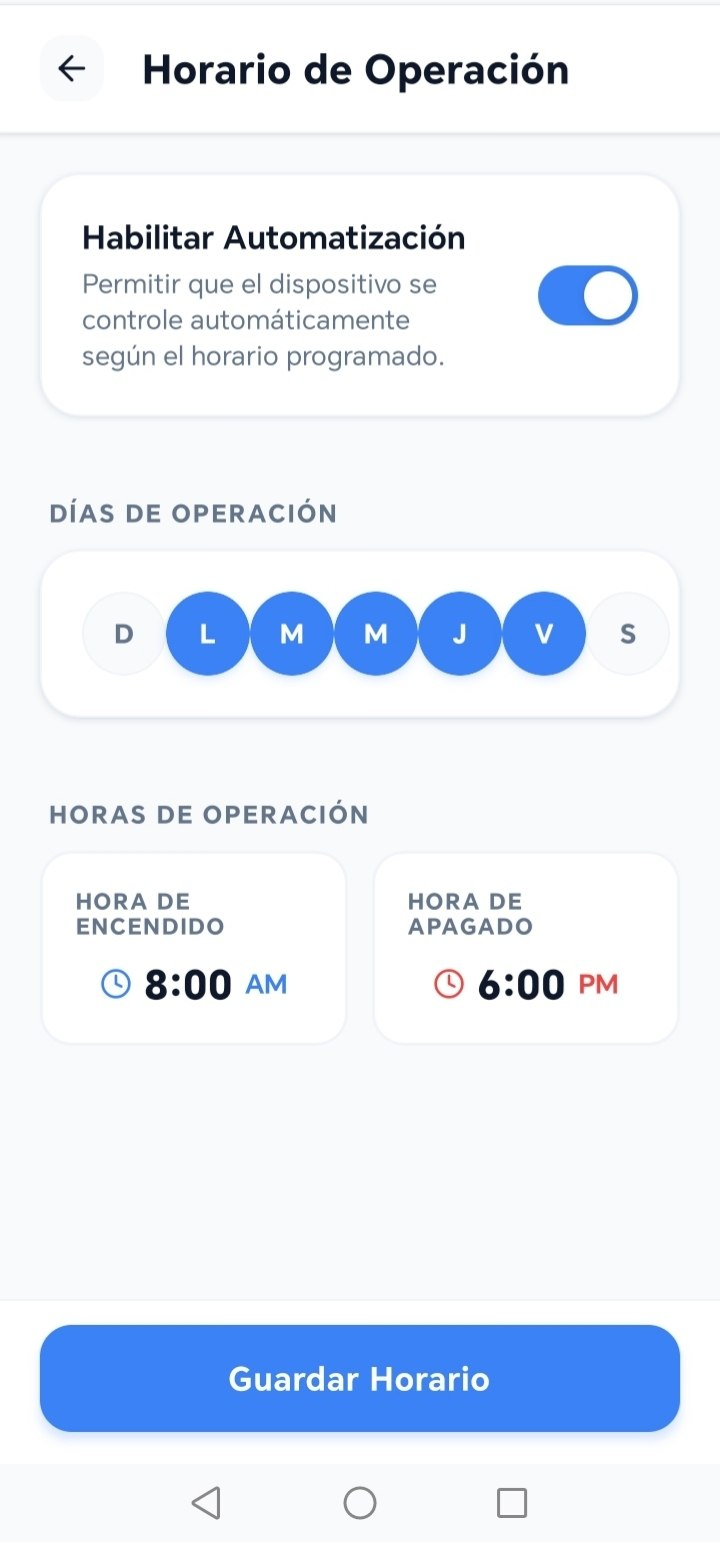
\includegraphics[width=0.28\textwidth]{../aplicacion_ss/ScheduleScreen.jpg}
    \caption{Configuración de Horarios}
    \label{fig:schedule_screen}
\end{figure}

Permite programar encendidos y apagados automáticos por días de la semana.

\subsection{Campos de configuración}
\begin{itemize}
    \item \textbf{Habilitar automatización:} Interruptor principal. Si está apagado, el resto de la pantalla se bloquea.
    \item \textbf{Días de operación:} Botones circulares para seleccionar los días de la semana (Dom, Lun, Mar, Mié, Jue, Vie, Sáb).
    \item \textbf{Hora de encendido:} Toque la tarjeta y deslice las ruedas para elegir hora, minutos y AM/PM.
    \item \textbf{Hora de apagado:} Igual que la hora de encendido.
    \item \textbf{Guardar horario:} Botón fijo en la parte inferior para almacenar la configuración.
\end{itemize}

% ==========================================
% SECCIÓN 9: HISTORIAL DE EVENTOS
% ==========================================
\section{Historial de Eventos}

\begin{figure}[H]
    \centering
    \begin{minipage}{0.35\textwidth}
        \centering
        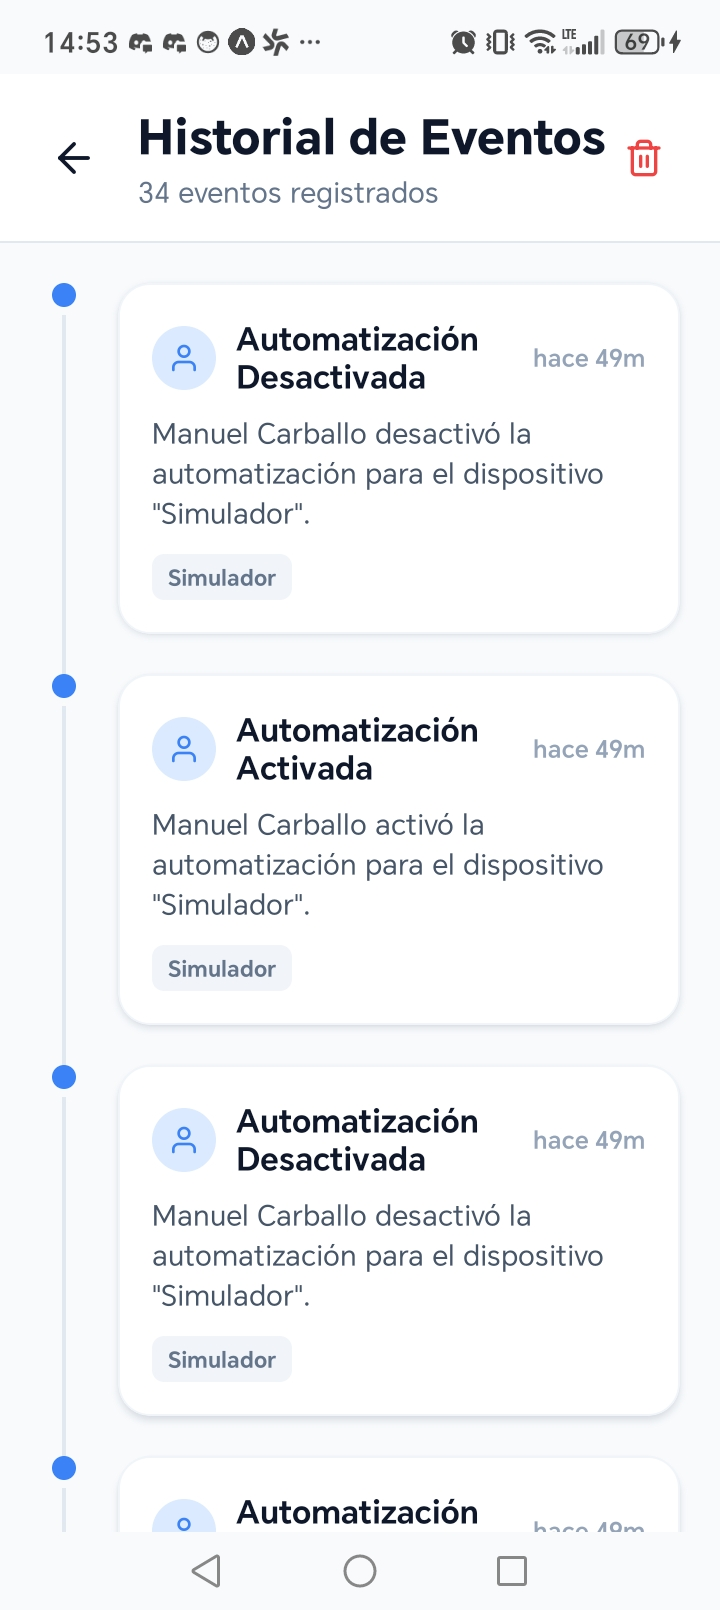
\includegraphics[width=0.8\textwidth]{../aplicacion_ss/Events_screen.jpg}
        \caption{Historial de Eventos}
        \label{fig:events_screen}
    \end{minipage}\hfill
    \begin{minipage}{0.6\textwidth}
        La aplicación guarda localmente los últimos \textbf{200 eventos} del sistema en una bitácora con línea de tiempo. Los eventos se clasifican en cinco niveles: acciones de usuario, del sistema, de la IA, advertencias y críticos. Cada evento muestra su tipo, descripción, dispositivo asociado y tiempo transcurrido.

        \smallskip
        En la esquina superior derecha hay un botón de papelera para borrar toda la bitácora tras confirmación.
    \end{minipage}
\end{figure}

% ==========================================
% SECCIÓN 10: NOTIFICACIONES
% ==========================================
\section{Notificaciones}

\begin{figure}[H]
    \centering
    \begin{minipage}{0.45\textwidth}
        \centering
        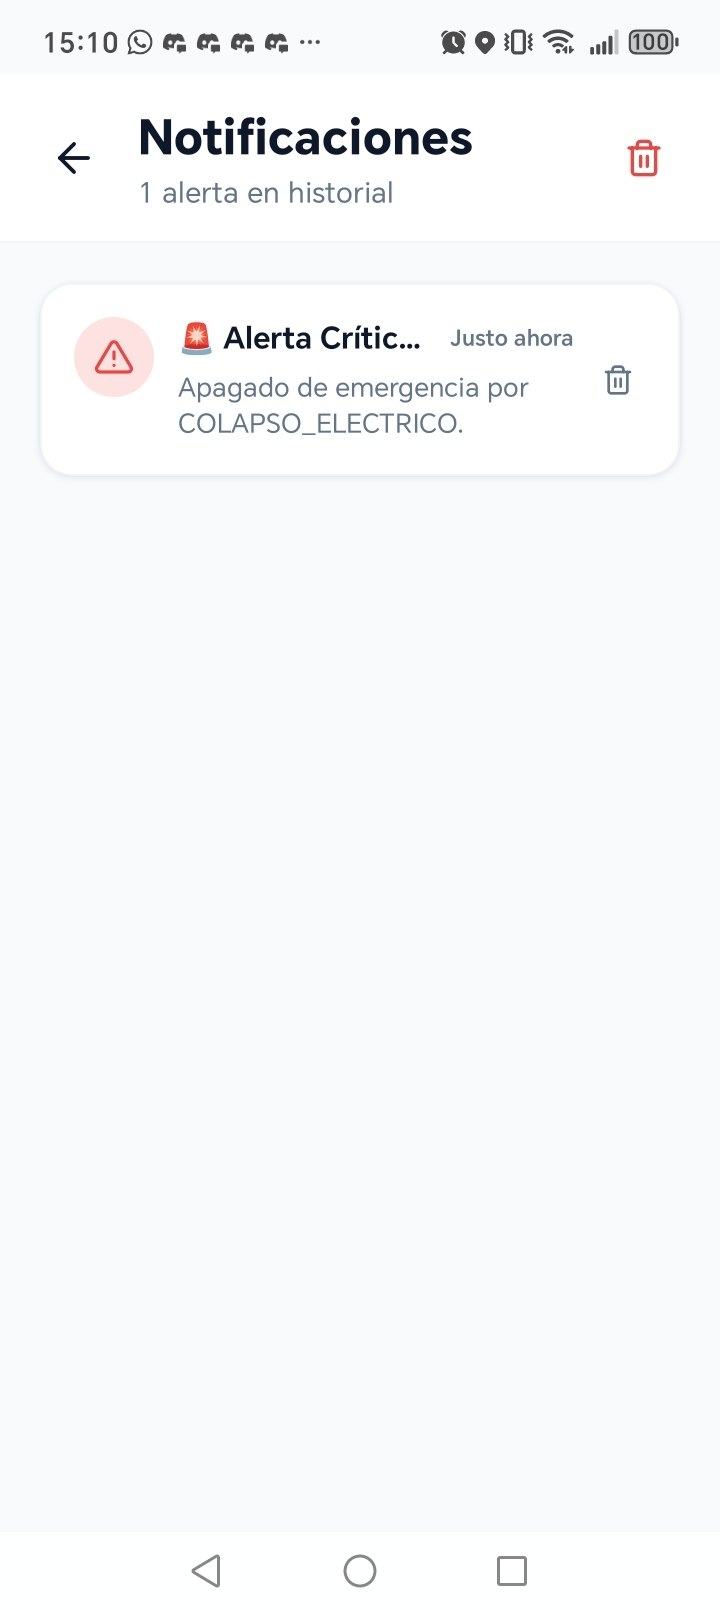
\includegraphics[width=0.55\textwidth]{../aplicacion_ss/NOTIFICATION_LIST.jpg}
        \caption{Lista de Notificaciones}
        \label{fig:notification_list}
    \end{minipage}\hfill
    \begin{minipage}{0.45\textwidth}
        \centering
        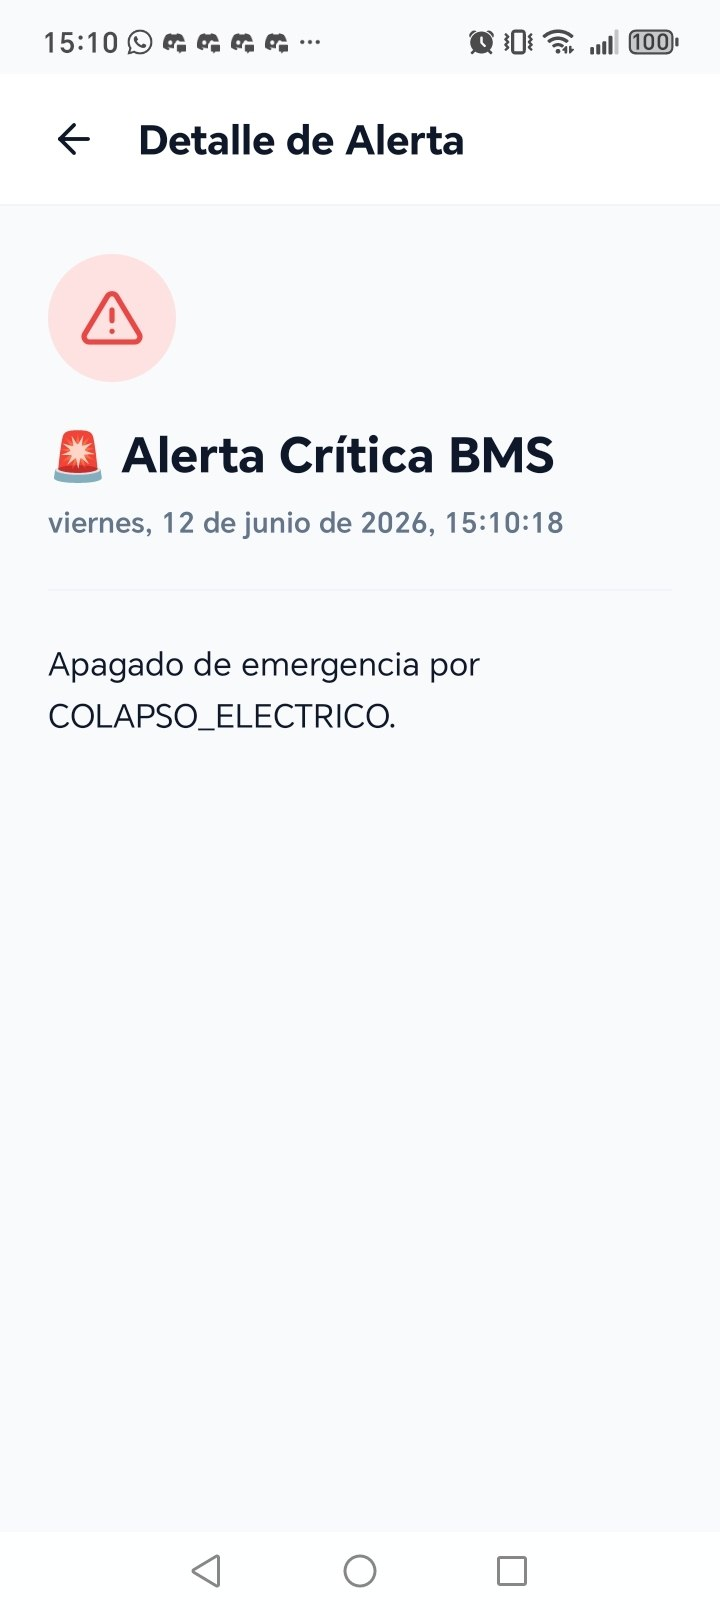
\includegraphics[width=0.55\textwidth]{../aplicacion_ss/NOTIFICATION_DETAILS.jpg}
        \caption{Detalle de Notificación}
        \label{fig:notification_detail}
    \end{minipage}
\end{figure}

La pantalla de notificaciones muestra el historial de alertas push recibidas. Acceda desde la campana del Dashboard.

\smallskip
Cada notificación incluye un icono de color según su tipo: rojo para alertas críticas (cortes de energía, emergencias), naranja para advertencias (consumo elevado, límites superados), morado para eventos de horario y azul para el resto.

\smallskip
Toque una notificación para ver su detalle completo. Las notificaciones no leídas se marcan automáticamente como leídas tras unos segundos. Use el botón de papelera en la esquina superior derecha para borrar todas, o elimine una por una con el ícono de papelera individual.

% ==========================================
% SECCIÓN 11: ANALÍTICAS
% ==========================================
\section{Analíticas}

\begin{figure}[H]
    \centering
    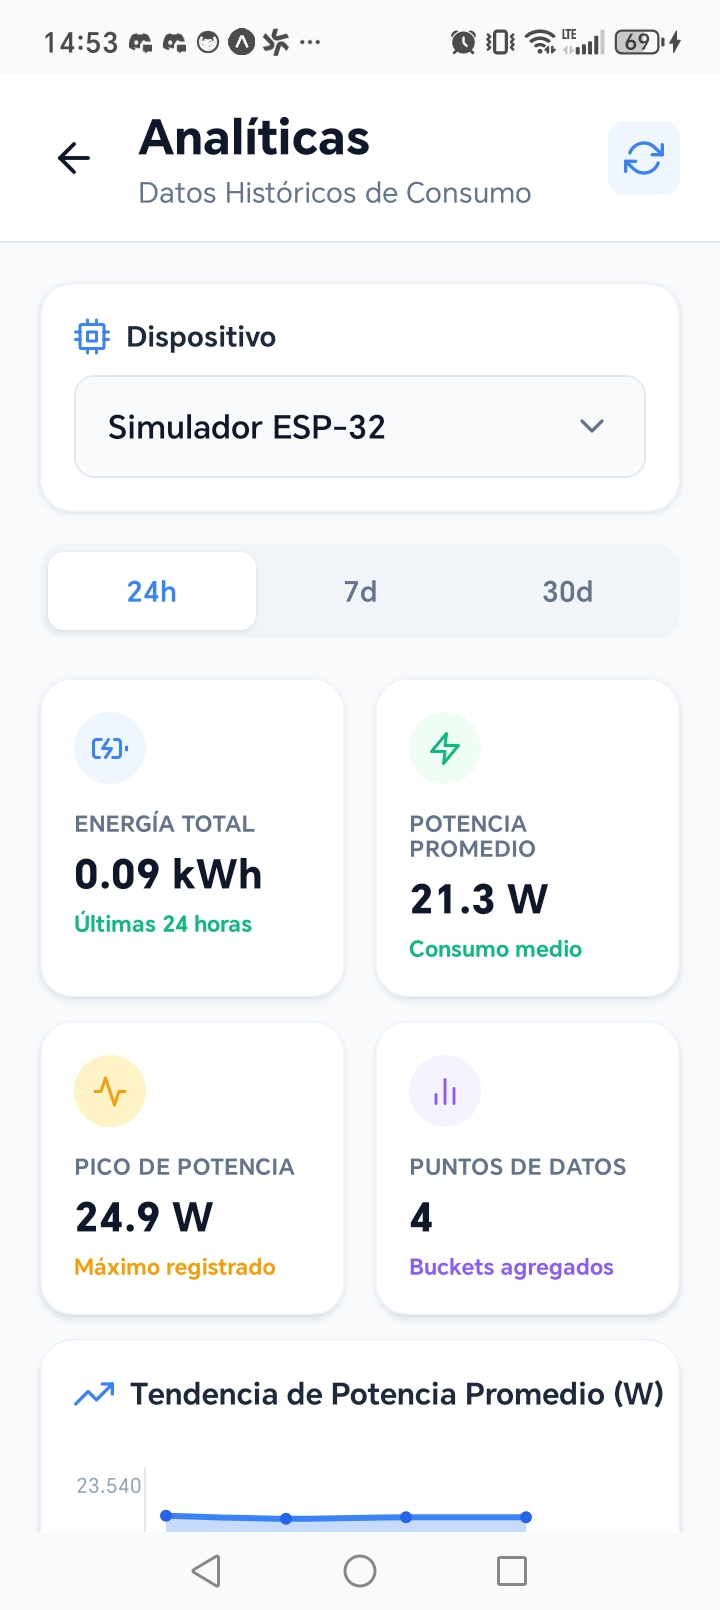
\includegraphics[width=0.28\textwidth]{../aplicacion_ss/ANALYTICS_1.jpg}
    \caption{Resumen de Consumo}
    \label{fig:analytics_1}
\end{figure}

\subsection{Selector de periodo y dispositivo}
\begin{itemize}
    \item \textbf{Periodo:} Elija \textbf{24h}, \textbf{7d} o \textbf{30d}.
    \item \textbf{Dispositivo:} Si tiene varios dispositivos, toque la tarjeta de selección para elegir cuál analizar.
\end{itemize}

\subsection{Tarjetas resumen}
\begin{itemize}
    \item \textbf{Energía Total:} Consumo acumulado en kilovatios-hora (kWh).
    \item \textbf{Potencia Promedio:} Nivel medio de potencia en vatios (W).
    \item \textbf{Pico de Potencia:} Valor máximo registrado (W).
    \item \textbf{Puntos de Datos:} Cantidad de registros analizados.
\end{itemize}

\subsection{Gráficos}

\begin{enumerate}
    \item \textbf{Tendencia de potencia:} Gráfico lineal del consumo promedio a lo largo del tiempo.
    \item \textbf{Distribución por nodo:} Gráfico circular (donut) que muestra qué porcentaje del consumo total corresponde a cada dispositivo. En el centro aparece la potencia total global.
    \item \textbf{Energía por periodo:} Gráfico lineal de la acumulación de vatios-hora (Wh).
\end{enumerate}

\subsection{Exportación}

\begin{figure}[H]
    \centering
    \begin{minipage}{0.45\textwidth}
        \centering
        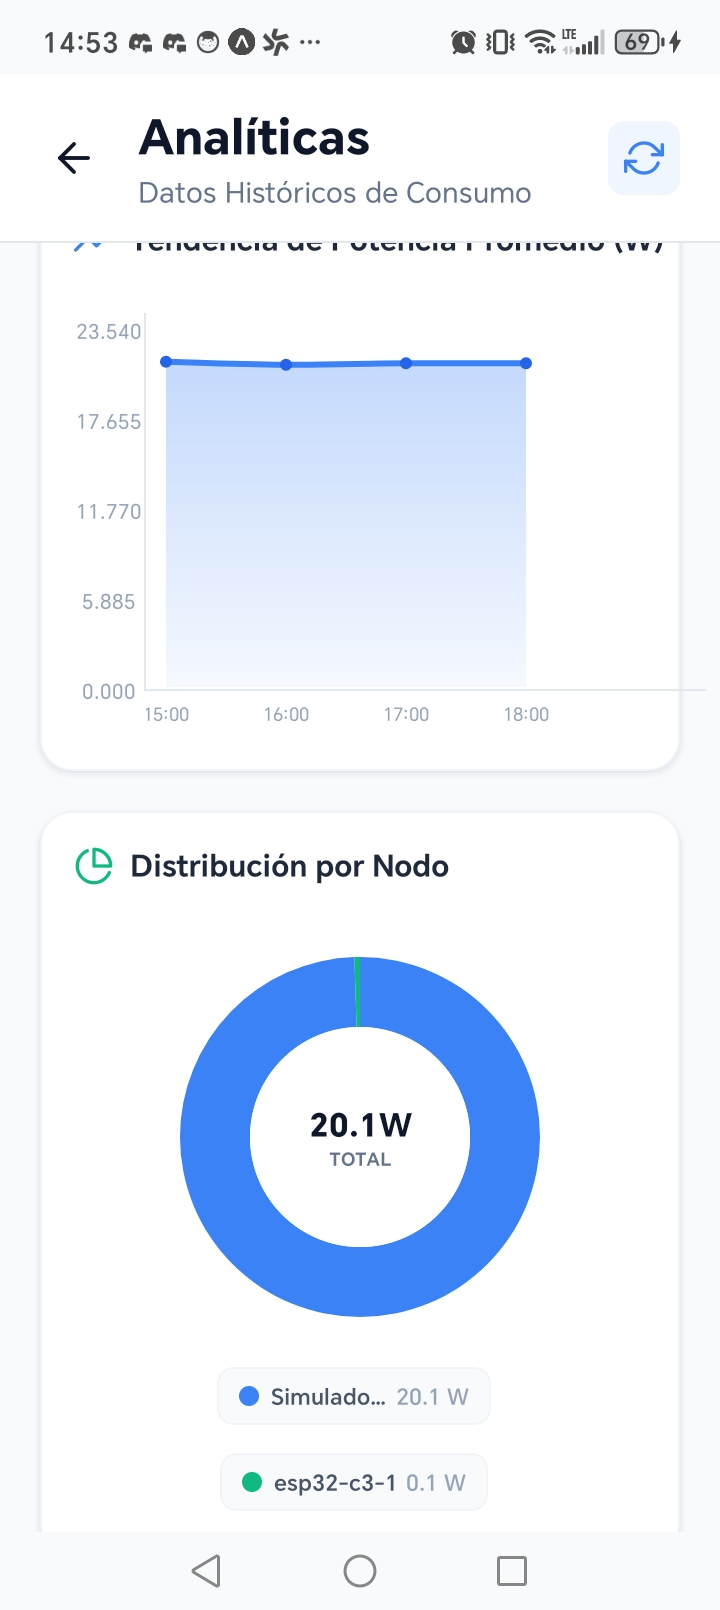
\includegraphics[width=0.55\textwidth]{../aplicacion_ss/ANALYTICS_2.jpg}
        \caption{Gráficos de Potencia y Distribución}
        \label{fig:analytics_2}
    \end{minipage}\hfill
    \begin{minipage}{0.45\textwidth}
        \centering
        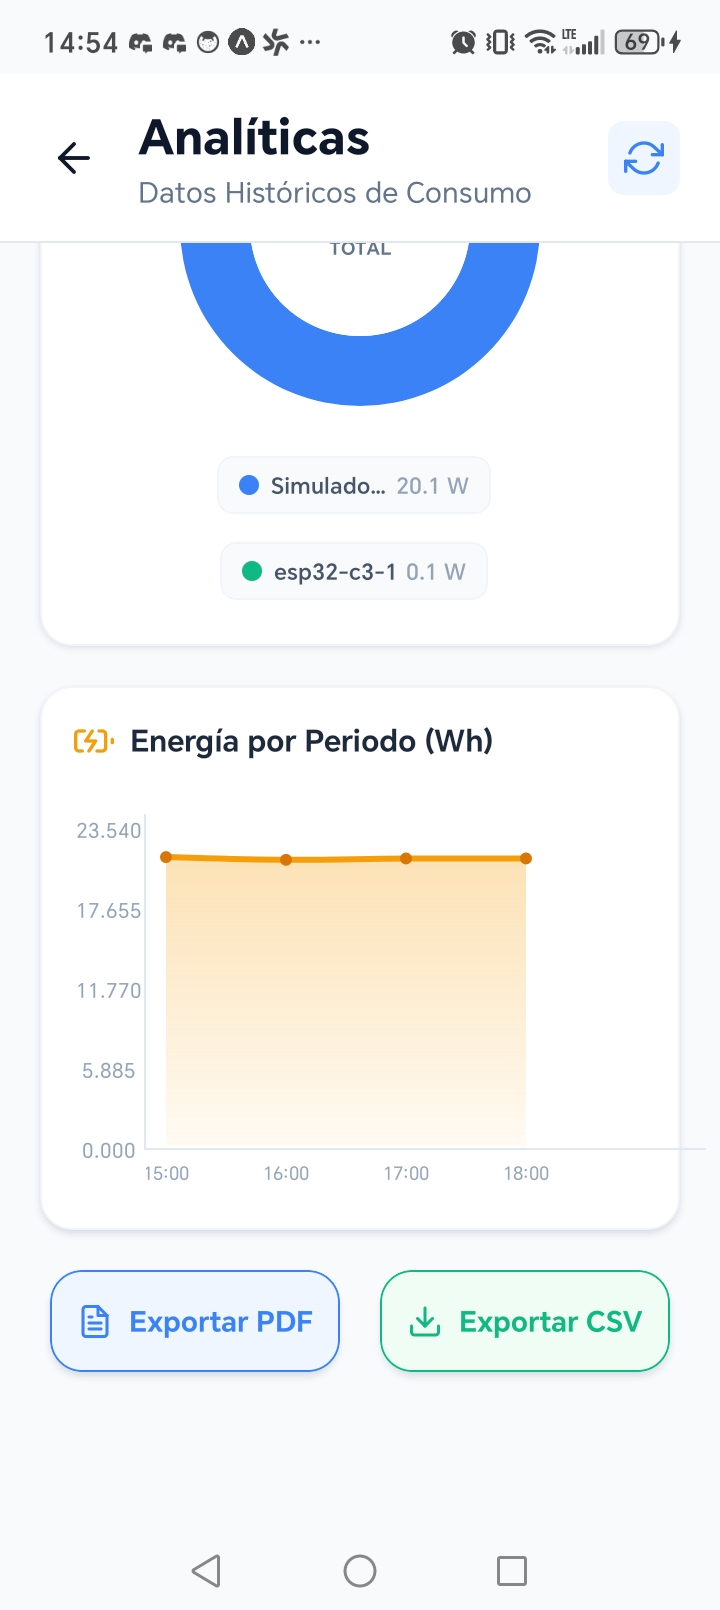
\includegraphics[width=0.55\textwidth]{../aplicacion_ss/ANALYTICS_3.jpg}
        \caption{Exportación de Reportes}
        \label{fig:analytics_3}
    \end{minipage}
\end{figure}

En la parte inferior hay dos botones:
\begin{itemize}
    \item \textbf{Exportar a CSV:} Archivo de texto separado por comas con los datos de telemetría.
    \item \textbf{Exportar a PDF:} Reporte visual con tablas y resumen, listo para compartir o imprimir.
\end{itemize}

% ==========================================
% SECCIÓN 12: AJUSTES
% ==========================================
\section{Ajustes}

\begin{figure}[H]
    \centering
    \begin{minipage}{0.45\textwidth}
        \centering
        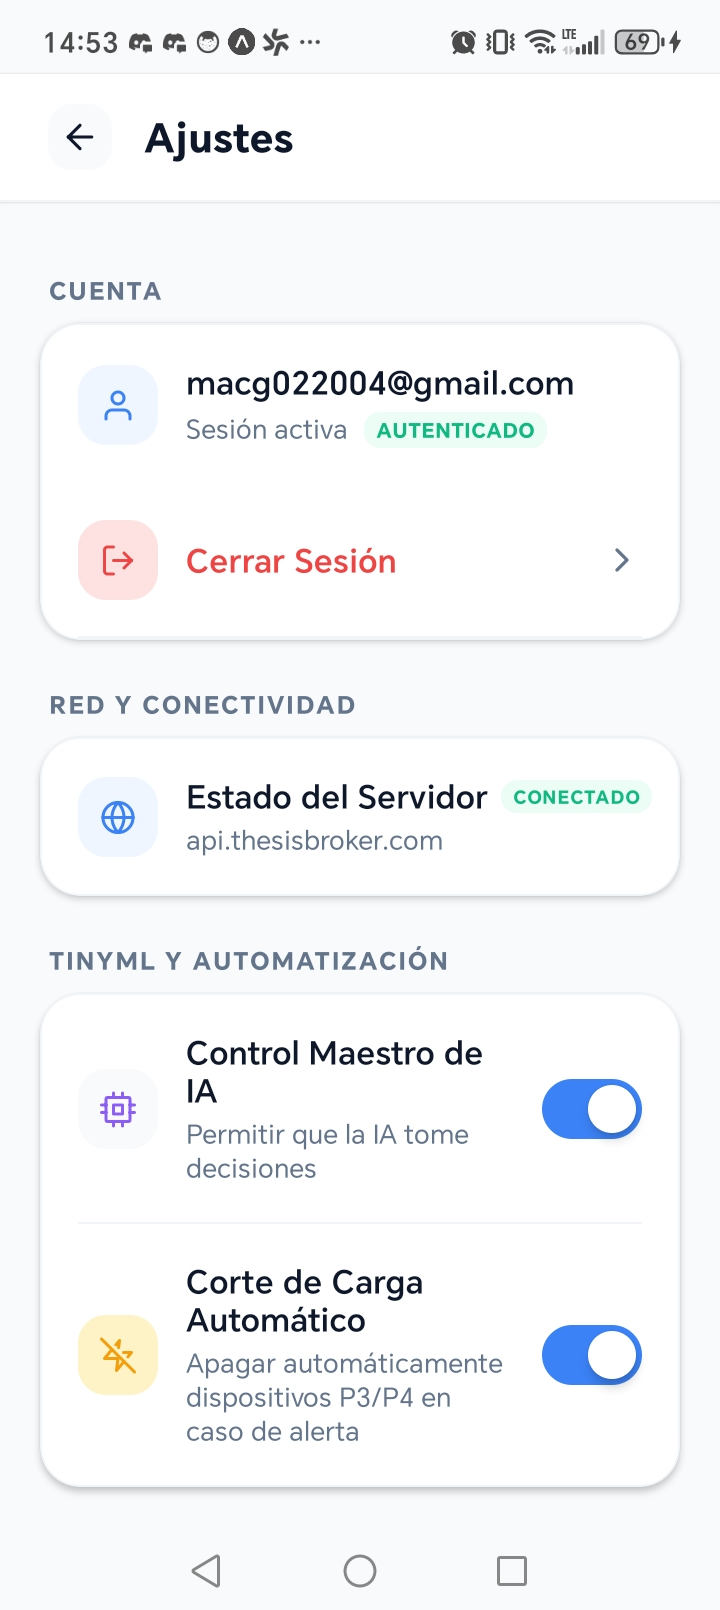
\includegraphics[width=0.55\textwidth]{../aplicacion_ss/SETTINGS_SCREEN_1.jpg}
        \caption{Pantalla de Ajustes --- Cuenta}
        \label{fig:settings_screen_1}
    \end{minipage}\hfill
    \begin{minipage}{0.45\textwidth}
        \centering
        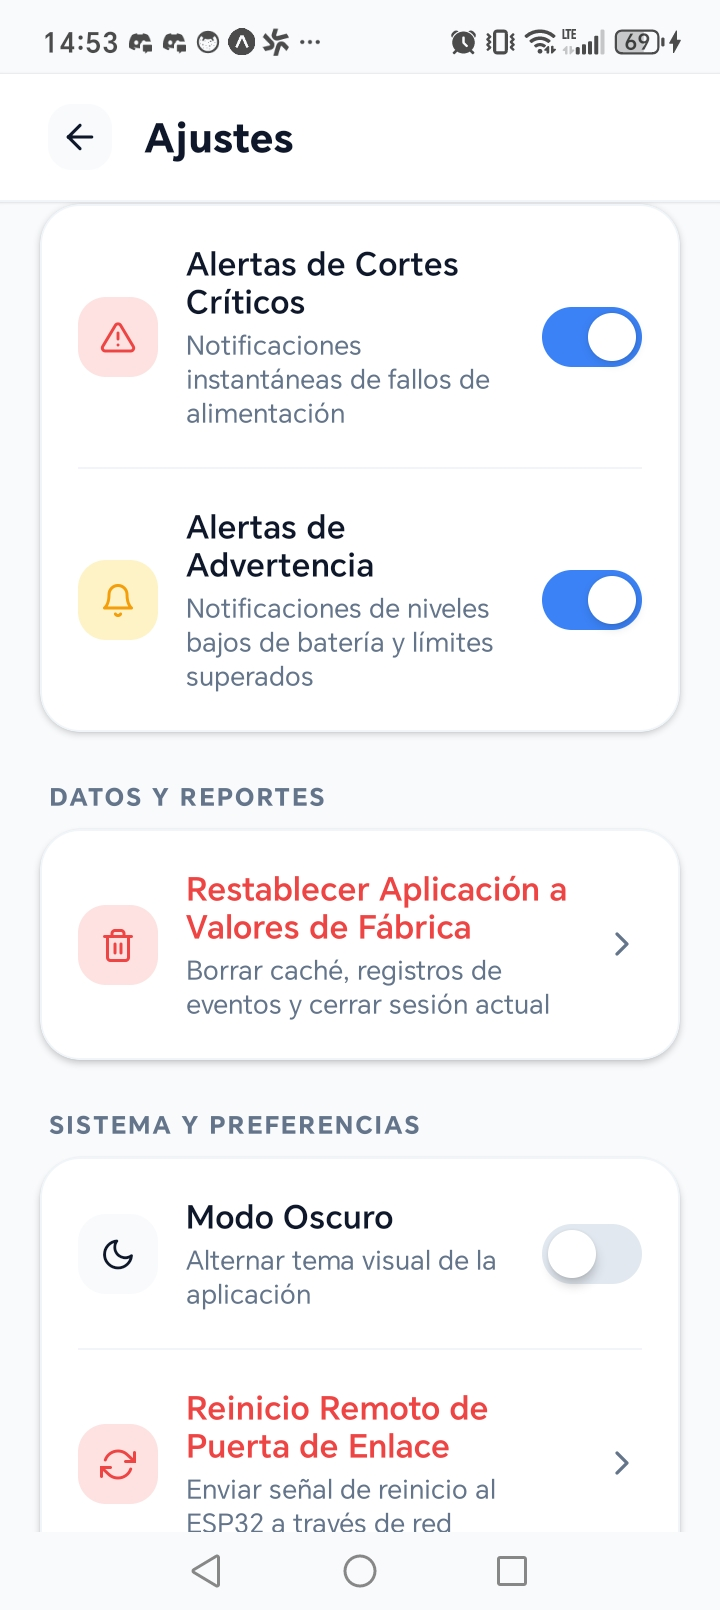
\includegraphics[width=0.55\textwidth]{../aplicacion_ss/SETTINGS_SCREEN_2.jpg}
        \caption{Pantalla de Ajustes --- Preferencias}
        \label{fig:settings_screen_2}
    \end{minipage}
\end{figure}

\subsection{Cuenta}
\begin{itemize}
    \item \textbf{Información de usuario:} Muestra el correo de la sesión activa.
    \item \textbf{Cerrar sesión:} Desvincula la cuenta del dispositivo móvil.
\end{itemize}

\subsection{Red y conectividad}
\begin{itemize}
    \item \textbf{Estado del servidor:} Indica si la aplicación puede comunicarse con el servidor central.
\end{itemize}

\subsection{Automatización}
\begin{itemize}
    \item \textbf{Control maestro de IA:} Activa o desactiva las decisiones automáticas del sistema.
    \item \textbf{Apagado de baja prioridad:} Si está activo, el sistema apaga automáticamente los dispositivos P3 cuando detecta un consumo riesgoso en la red.
\end{itemize}

\subsection{Alertas y notificaciones}
\begin{itemize}
    \item \textbf{Cortes críticos:} Notificaciones de apagados de emergencia y desconexiones.
    \item \textbf{Advertencias:} Notificaciones de niveles de riesgo y límites superados.
\end{itemize}

\subsection{Sistema y preferencias}
\begin{itemize}
    \item \textbf{Modo oscuro:} Cambia entre tema claro y oscuro.
\end{itemize}

\subsection{Datos y reportes}
\begin{itemize}
    \item \textbf{Restablecer aplicación:} Borra el historial local, la caché y cierra la sesión. Use esta opción con precaución.
\end{itemize}

\end{document}
